\subsection{Algorithm 1}
The first algorithm is straightforward and rudimentary. Like the description of the model stated the simulation first checks if it can add balloons to the system. After doing so each balloon in the system uses the following logic to determine whether it should move or not:

\begin{algorithm}[H]
  \If{Multiple balloons same spot}{
 	\If{At bottom layer} 
 	{Go up}
 	\ElseIf{At top layer}  	
 	{Go Down}
 	\Else  	
 	{Choose direction at random}
 }
 \Else
 {Stay in current layer}
 \caption{Control Algorithm 1}
 \label{alg1}
\end{algorithm}

This algorithm has an obvious downside since as it contains an element of random, which is usually not helpful in a control algorithm. Nevertheless, it spreads the balloons thoroughly around the grid relatively fast. The control over the grid is however limited and this would not be a suitable solution if the end goal is to provide stable coverage.

This algorithm might however be utilized as a part of a larger more complex algorithm. At the beginner stages of the balloon's life cycle it could prove helpful to get the balloon out of that first wind layer and join the huddle.  

\subsection{Algorithm 2}
This algorithm is a step towards a more complex control algorithm. Some minor logic replaces the random generator in the previous solution. 

\begin{algorithm}[H]
  \If{Multiple balloons same spot}{
  Calculate projections\;
  
 	\If{optionUp < optionDown} 
 	{Go up}
 	\Else
 	{Go down}

 }
 \Else
 {Stay in current layer}
 \caption{Control Algorithm 2}
 \label{alg2}
\end{algorithm}

The balloon fetches the wind vectors from neighbouring wind layers and uses them to weigh its options. It computes the number of balloons occupying three different cells:
\begin{enumerate}
\item The cell to which the balloon's current wind layer will move it.
\item The cell to which the the wind layer above the balloon's current wind layer would move it.
\item The cell to which the the wind layer below the balloon's current wind layer would move it.
\end{enumerate}

The algorithm then determines which option has the cell with the lowest number of balloons and chooses that direction.
\begin{figure}
\centering
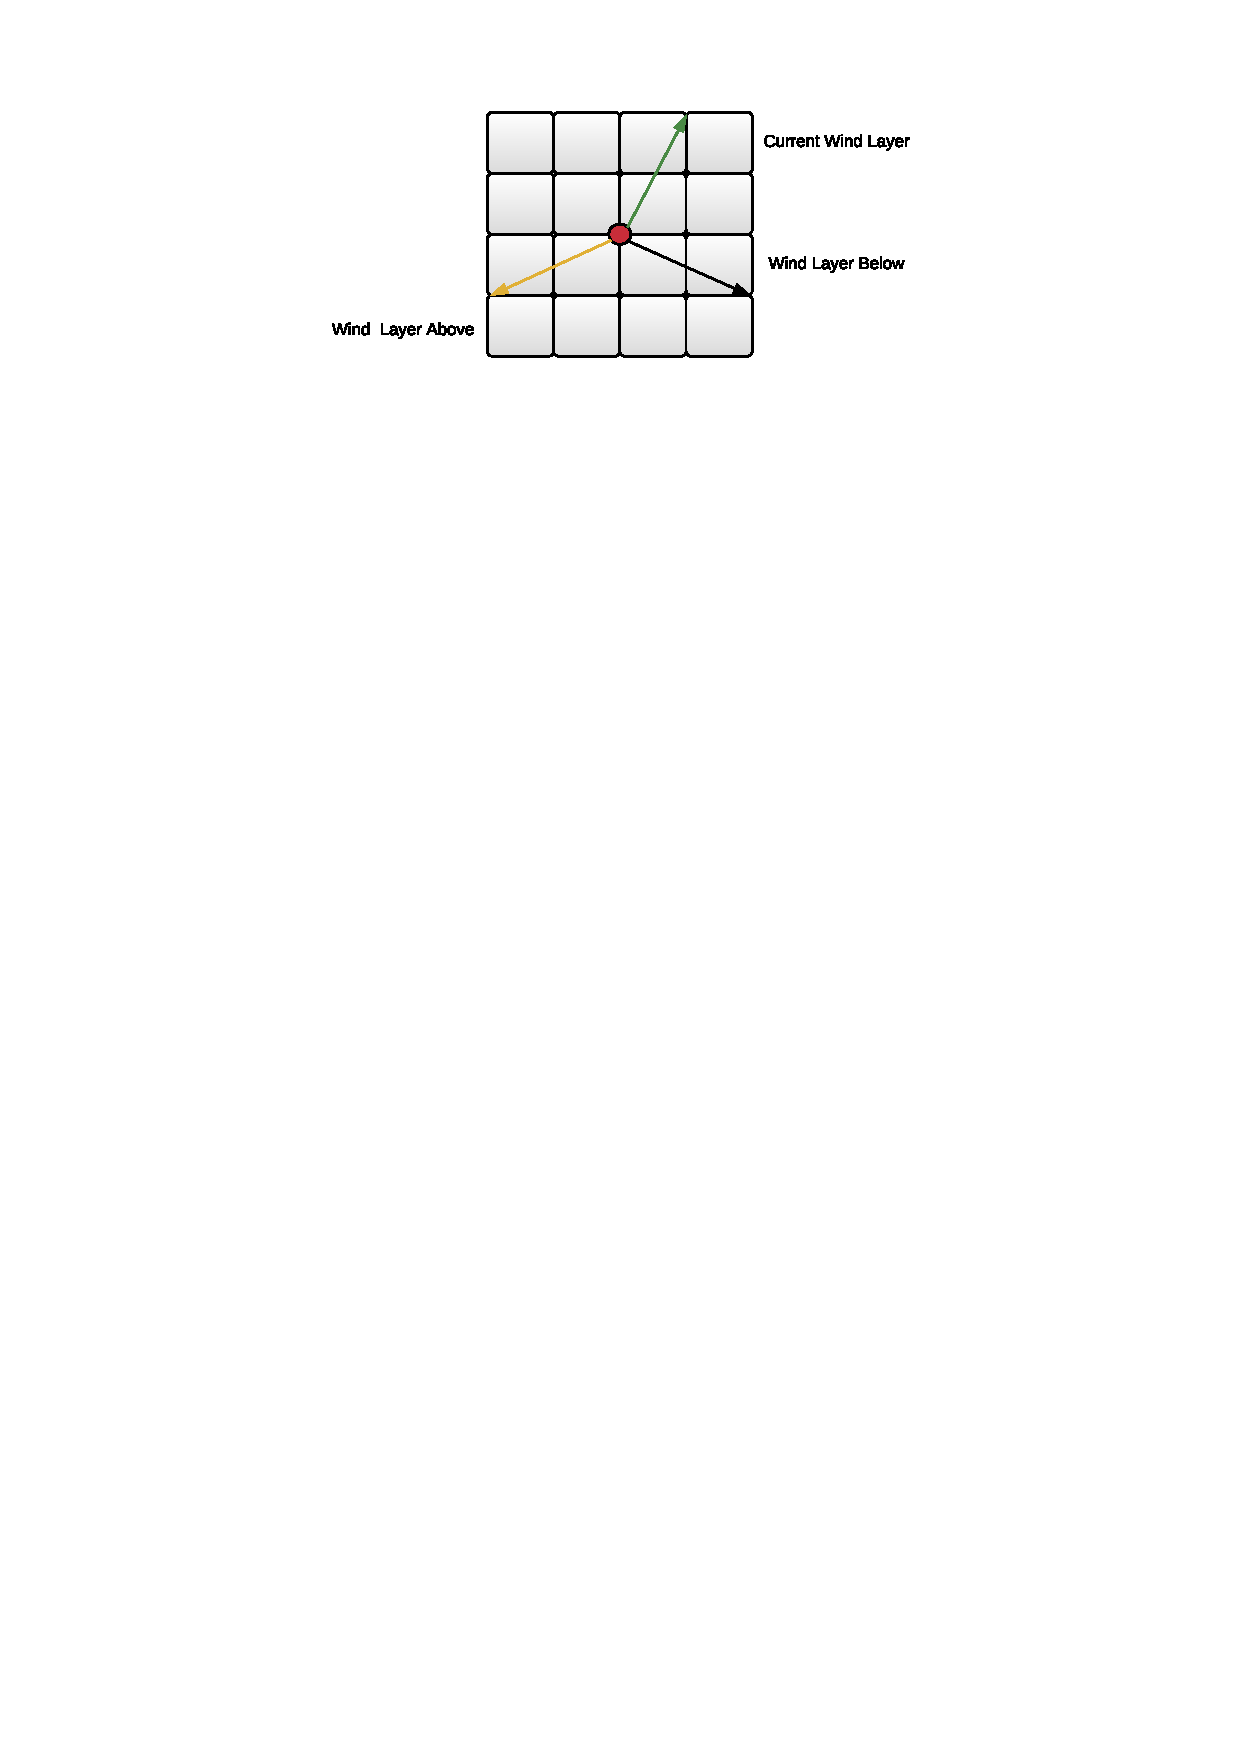
\includegraphics[width=0.8\textwidth,trim= 4cm 23cm 4cm 1cm,clip]{graphics/Projections.pdf}
\caption{Calculate projections}
\label{fig:projections}
\end{figure}

\begin{figure}
\centering
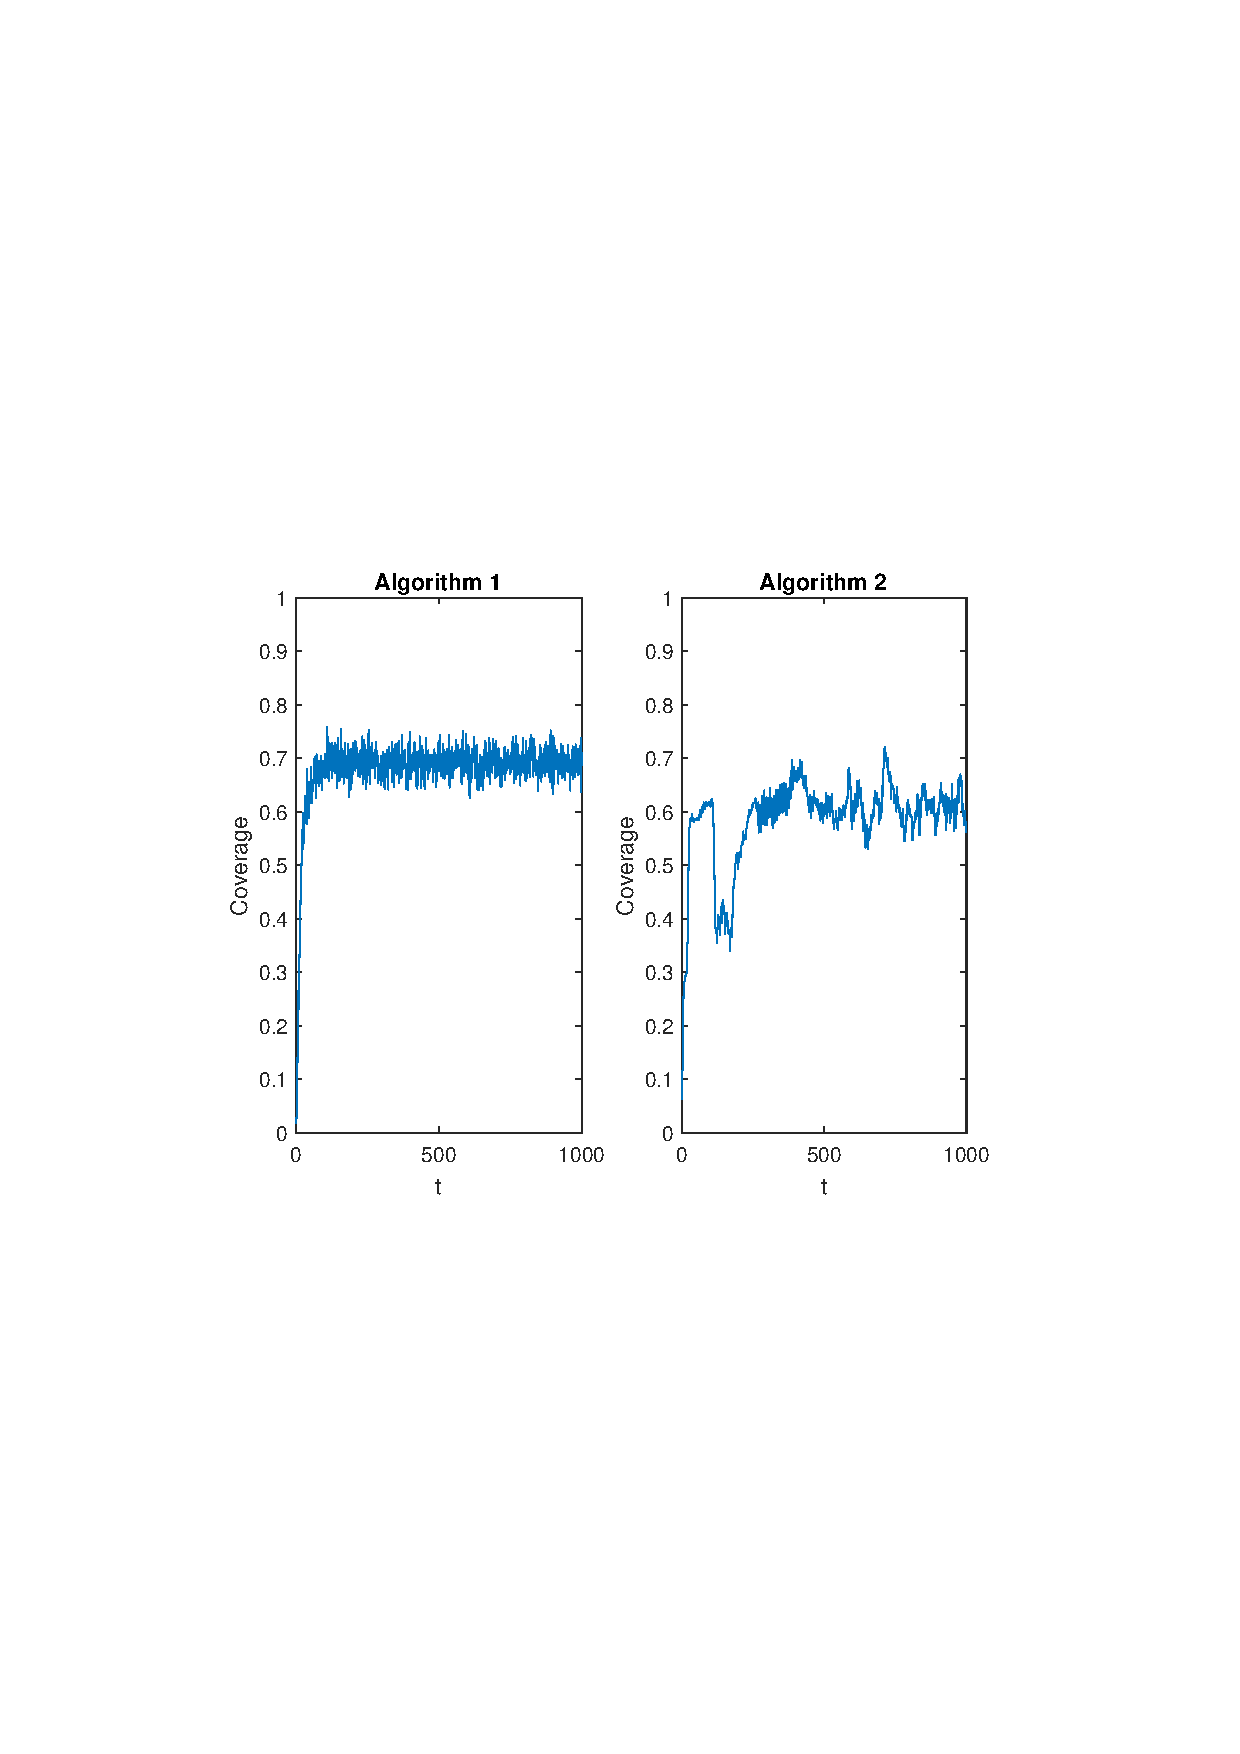
\includegraphics[scale=0.7, trim={3cm 10cm 4cm 9cm},clip]{graphics/coverage_alg1_vs_alg2_1000steps_LIFETIMELONG.pdf}
\caption{Algorithm 1 vs. Algorithm 2 in 1000 steps with an infinite lifetime of each balloon}
\label{fig:alg1vsalg2}
\end{figure}
It is interesting to see that Algorithm 1 outperforms Algorithm 2 when it comes to coverage and stability. Not only did Algorithm 1 reach higher coverage like Figure \ref{fig:alg1vsalg2} clearly shows but was also more stable. Multiple simulations were run and the each output graph was from Algorithm 1 was exactly the same while the graph for Algorithm 2 was changed with every each simulation. The figure of the comparison shows a typical output for both algorithms.

\begin{figure}
\centering
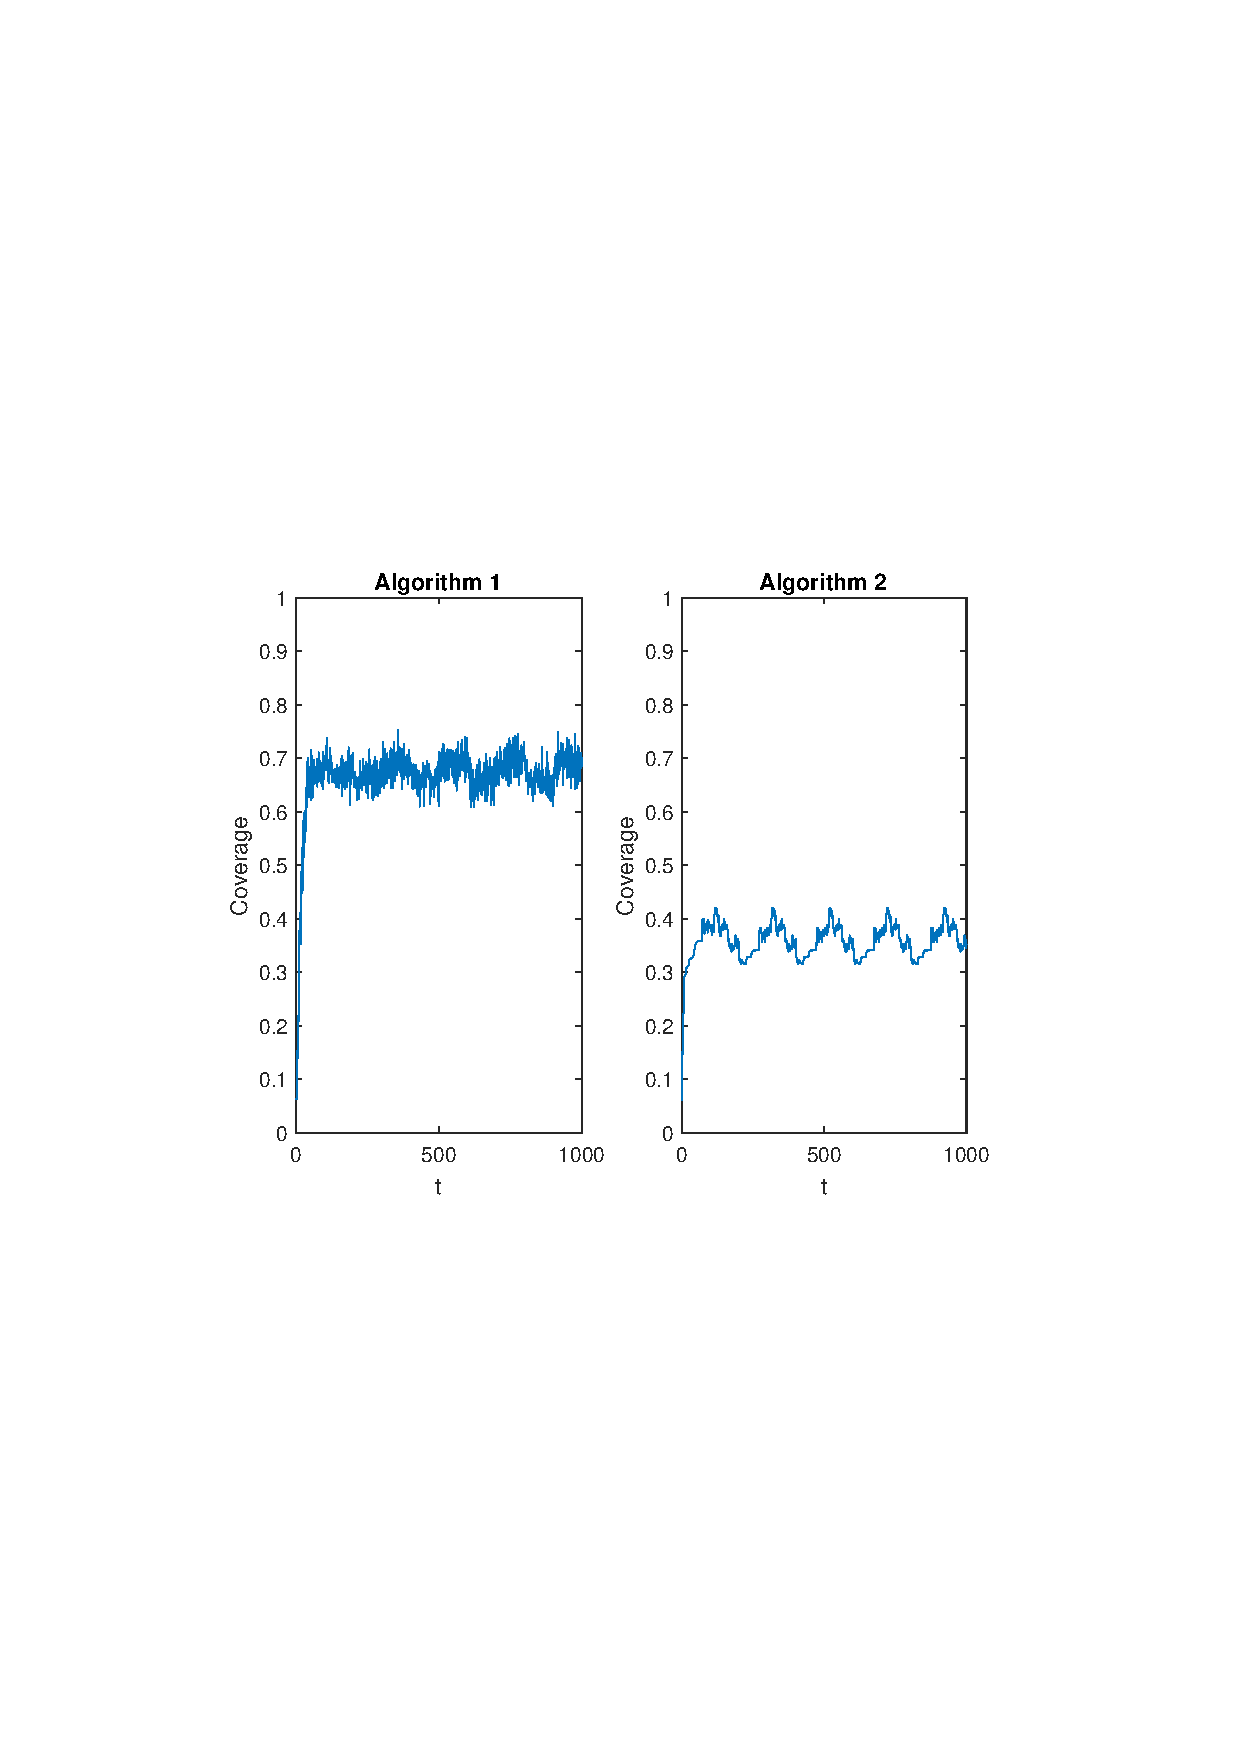
\includegraphics[scale=0.7, trim={3cm 10cm 4cm 9cm},clip]{graphics/coverage_alg1_vs_alg2_1000steps_LIFETIME200.pdf}
\caption{Algorithm 1 vs. Algorithm 2 in 1000 steps with lifetime 200}
\label{fig:alg1vsalg2_200}
\end{figure}

Algorithm 1 also does a better job of maintaining the coverage while repopulating the system, but that can be seen in Figure \ref{fig:alg1vsalg2_200}. Each 200 steps a balloon is removed, and recreated at coordinates (0,0). Like mentioned earlier, Algorithm 1 does any excellent job of spreading the balloons quickly and thoroughly so this lifetime heavily favours that algorithm. Algorithm 2 is never able to spread the balloons well enough before it has to start all over again.


\subsection{Algorithm 3}
The third algorithm is a modification of the second algorithm and introduces a new feature to the balloon. The second algorithm based its decision on the number of balloons in the neighbouring cells, and which wind layer would blow it to the most vacant cell. 

The third algorithm communicates with the balloons in its communication radius and makes the decision based on the data it receives. This is done through a private function. The function creates a list of all balloons within the communication radius. Then each of the balloons in that list counts it own neighbours and returns the value. The balloon with the fewest number of neighbours is deemed as a critical point. 

\begin{figure}[H]
    \centering
    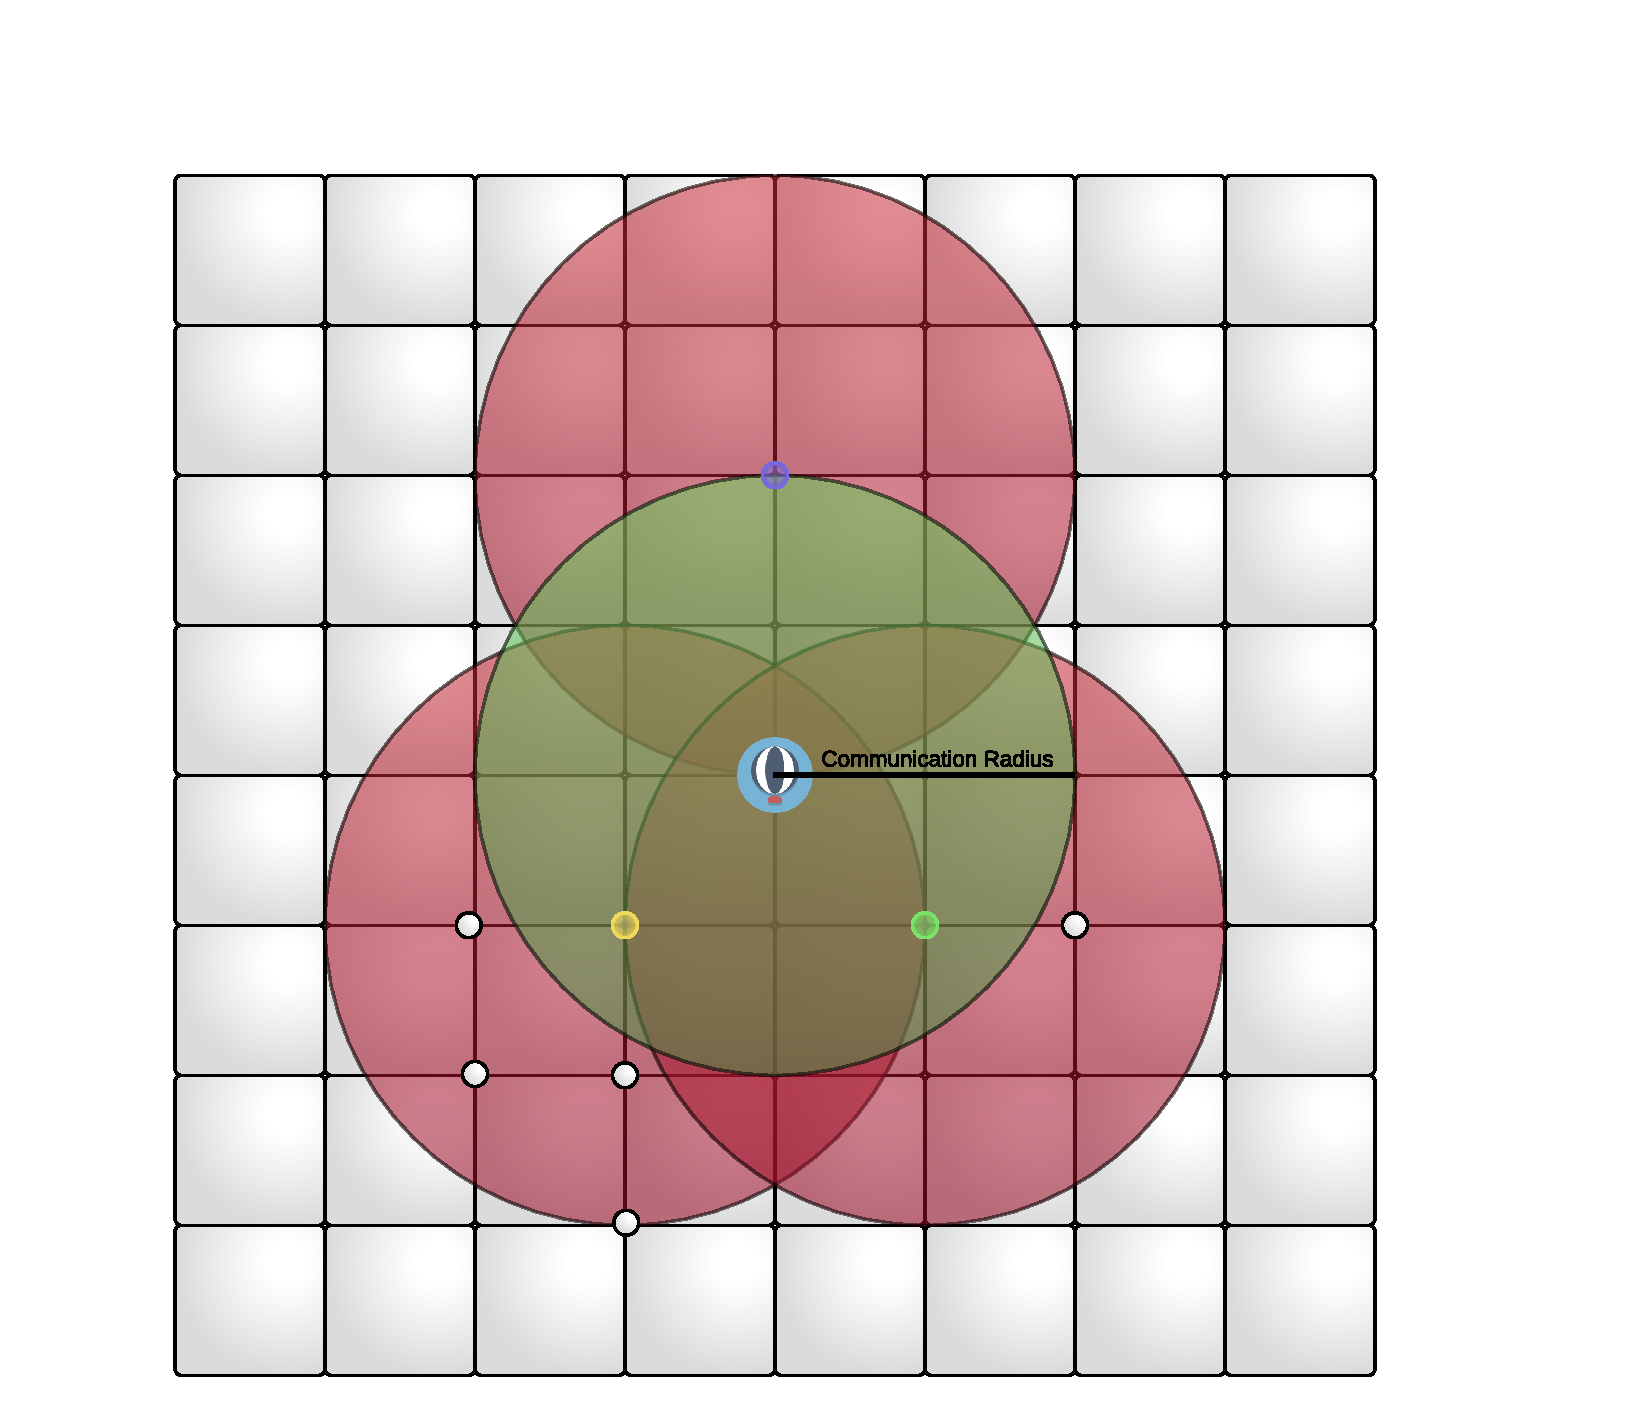
\includegraphics[scale=0.5]{graphics/criticalPointimproved.pdf}
    \caption{Critical point computed. The blue point will be deemed critical}
    \label{fig:criticalf}
\end{figure}

Figure \ref{fig:criticalf} shows an example of calculations of a critical point. The main balloon has three neighbours represented with different colours. Each of the three neighbours has its own number of neighbours. The yellow, green and purple balloons each have 6, 3 and 1 neighbours respectively. This means that the coordinates of the purple balloon are returned as a critical point.

Algorithm 3 is also the first algorithm to explore more than just the windlayer above and below, but the entire stratosphere. To be able to navigate towards that layer, a  \textit{nextLayer} attribute has been introduced to the balloon object. When a balloon is moved between layers, this variable is used to determine if the vertical movement should be stopped or not, i.e if the balloon has reached is destined layer or not.

\begin{algorithm}[H]
  \If{More than 1 balloon at current space}{
  Find point c (critical point)\\
  
    Calculate projectedPair (pp) for current layer\\
    
    smallestPP = distance(pp, c)\\
  \ForAll{WindLayer wl : stratosphere} {
  
  Calculate projectedPair (pp) 
  
  Calculate distance(pp,c)
  
  \If{pp$<$smallestPP}{wl is chosen as NextLayer}}
  \EndFor
  
  NextLayer set as attribute of balloon
  
\If{NextLayer is above CurrentLayer}{
goUp()
}
\Else{
goDown()
}

 }
 \Else
 {Stay in current layer}
 \caption{Control Algorithm 3}
 \label{alg3}
\end{algorithm}

\begin{figure}
    \centering
    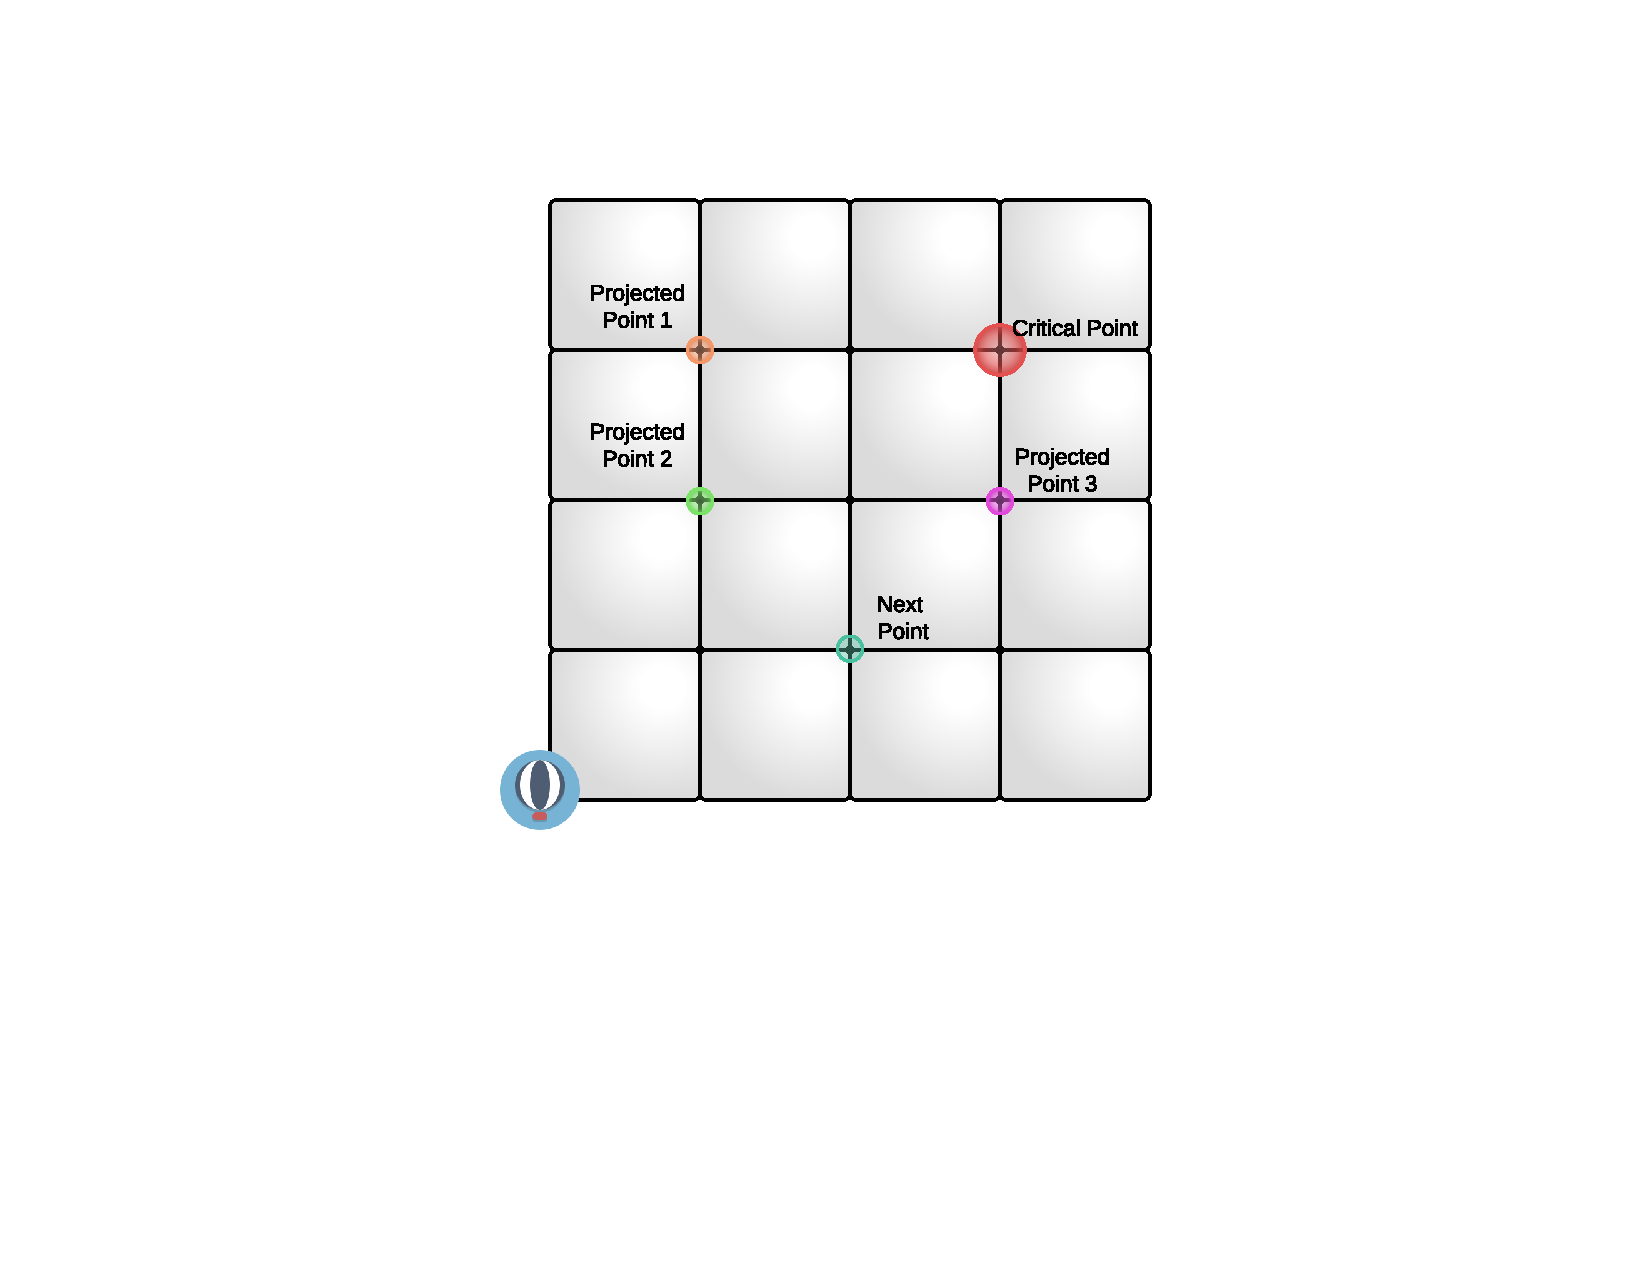
\includegraphics[width=\textwidth, trim=5cm 7cm 5cm 3.3cm, clip]{graphics/projectedPoints.pdf}
    \caption{Critical point computed}
    \label{fig:critical}
\end{figure}

When a critical point has been determined, a projection point is created for all wind layers in the stratosphere. This is represented in figure \ref{fig:critical}. The distance $d$ between each projection point ($x_p, y_p$) and the critical point ($x_c,y_c$) is calculated with the following formula:

\begin{align}
d = \sqrt{(x_c-x_p)^2+(y_c-y_p)^2} \notag
\end{align}

\subsection{Algorithm 3s}
Algorithm 3 was the first algorithm to offer movement between multiple layers at a time. The transition does not happen instantaneously since a balloon has a fixed vertical speed. This means that a balloon can be interrupted in its transition, and the destination layer changed before the balloon reaches its target. Algorithm 3s is a minor twist on Algorithm 3 as it only adds one criteria. No decision is made by balloons that are already in motion:

\begin{algorithm}[H]
\ForAll{Ballon b : balloons}{
\If{b is not moving vertically}{applyDecision3(b)}
}
\caption{Control Algorithm 3s}
\label{alg:3s}
\end{algorithm}

Figures \ref{fig:alg3vsalg3s_long} and \ref{fig:alg3vsalg3s_200} show the performance of the algorithms, first with an infinite lifetime of all balloons. There the coverage is fairly similar once the simulation has created all balloons. The second simulation is with lifetime of 200 steps. Algorithm 3 does a decent job of keeping stable, while the coverage with Algorithm 3s plunges every 200 steps in the simulation. With this extra criteria in place it makes the algorithm slower to respond to changes since each balloon does not respond while it is currently undertaking a change in altitude. The conclusion is that 

\begin{figure}
\centering
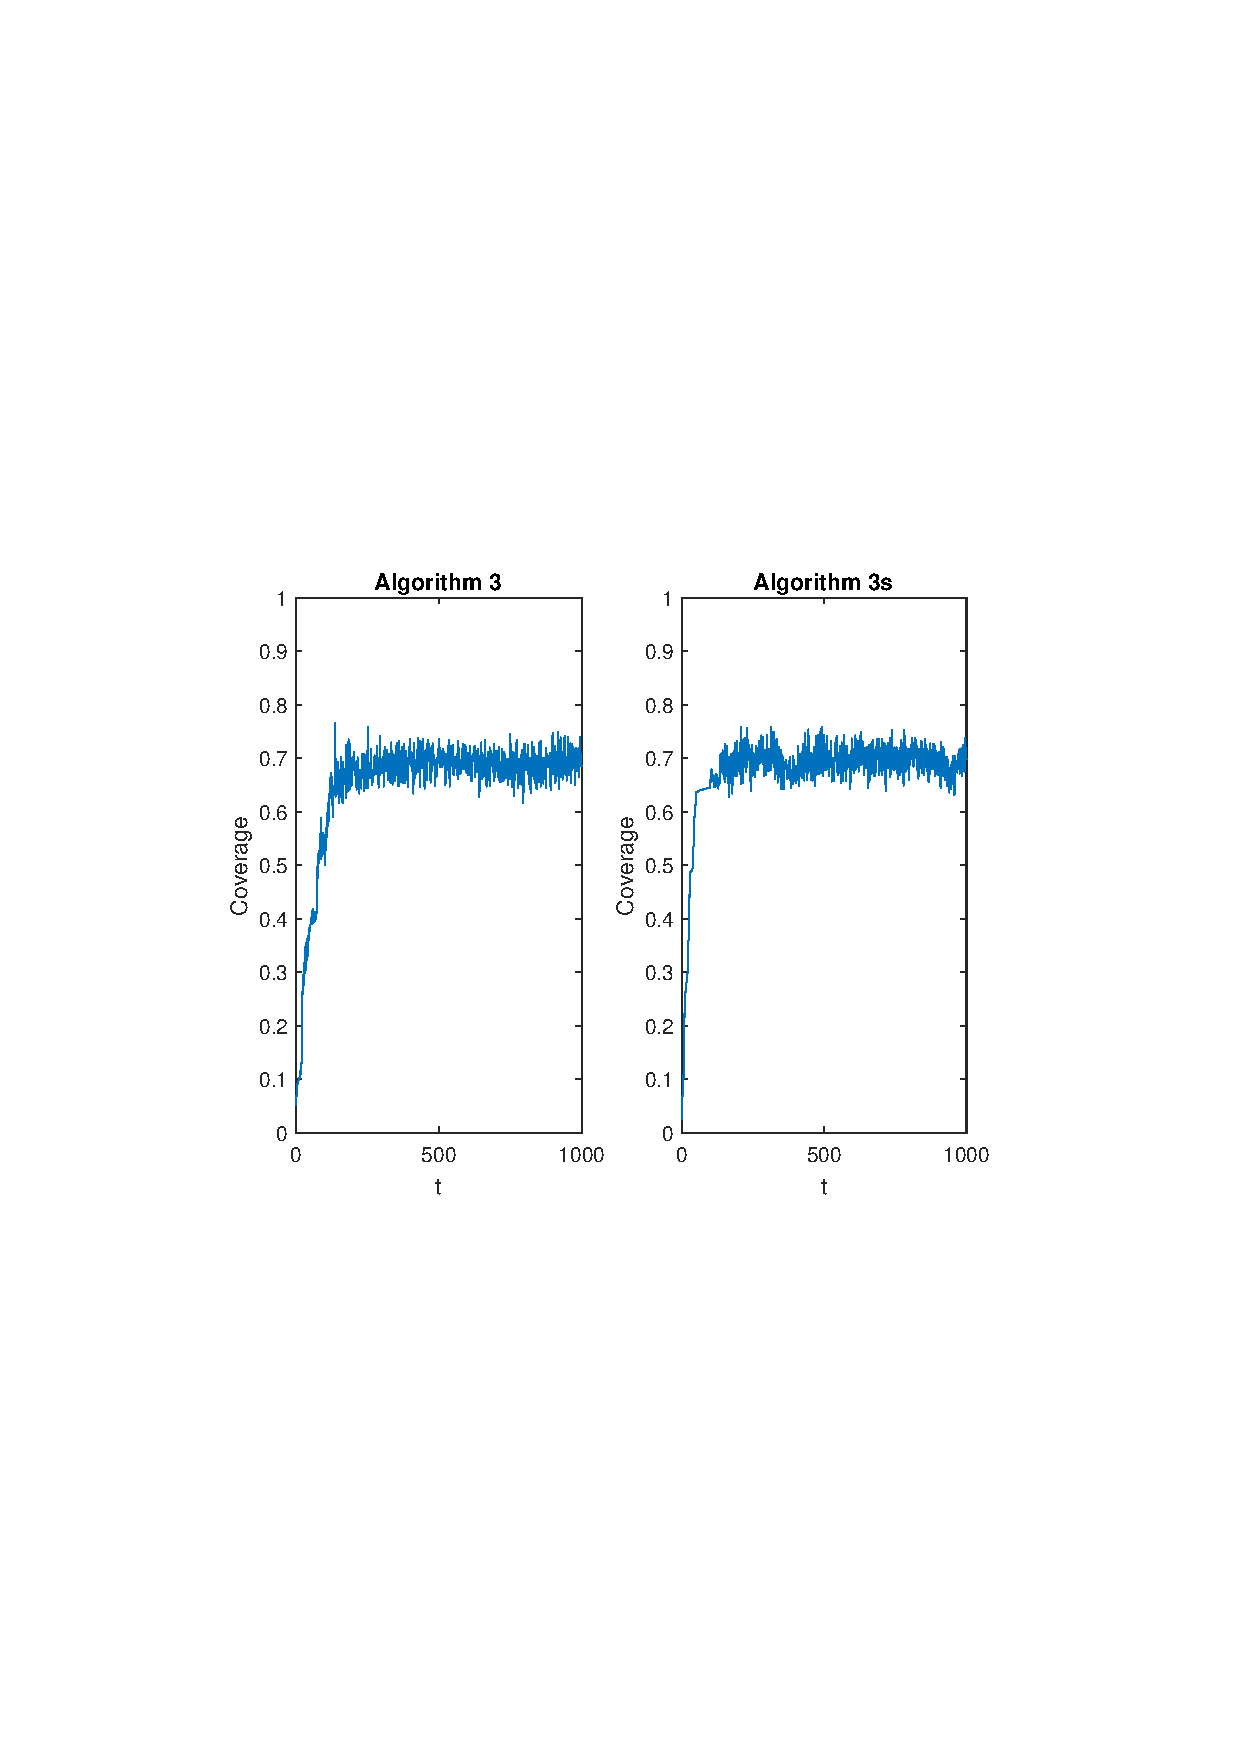
\includegraphics[scale=0.7, trim={3cm 10cm 4cm 9cm},clip]{graphics/coverage_alg3_vs_alg3s_1000steps_LIFETIMELONG.pdf}
\caption{Algorithm 3 vs. Algorithm 3s in 1000 steps with an infinite lifetime of each balloon }
\label{fig:alg3vsalg3s_long}
\end{figure}
\begin{figure}
\centering
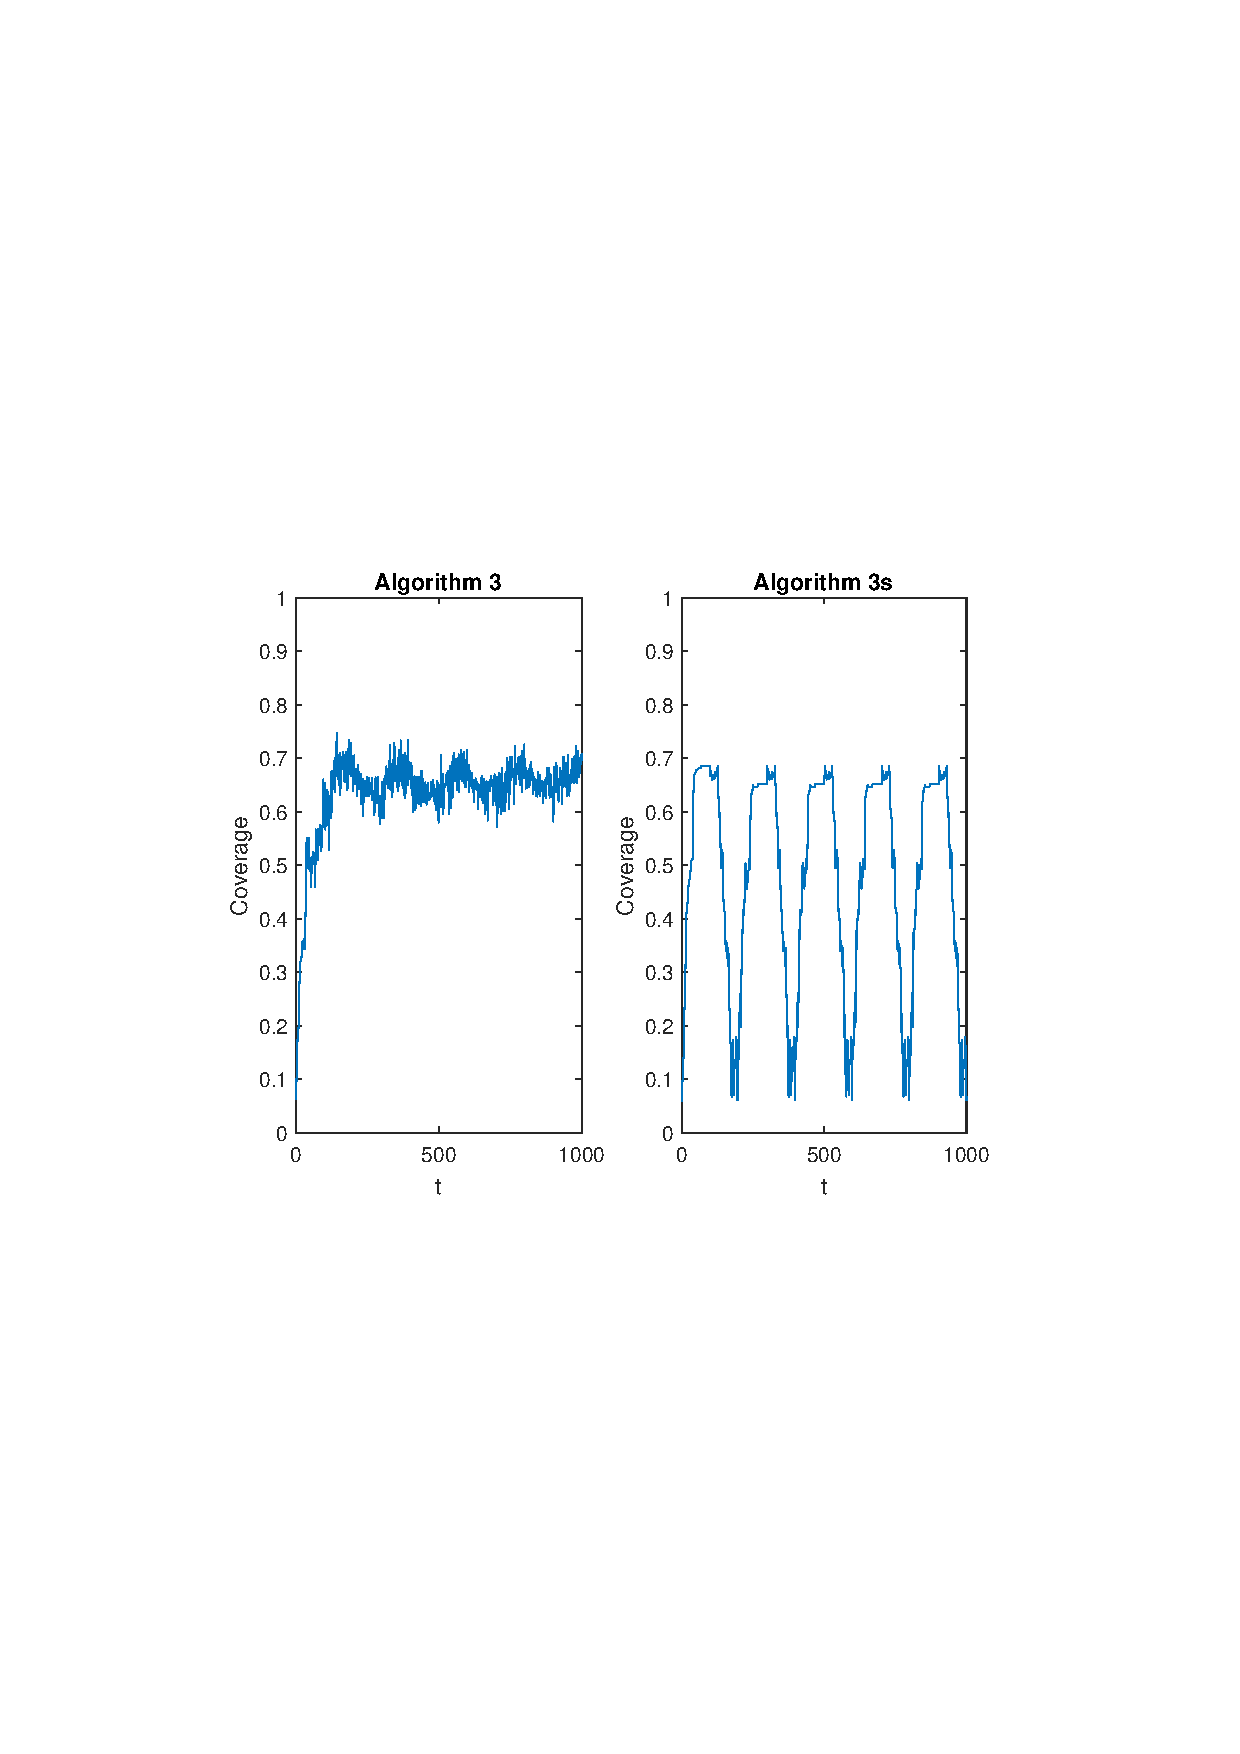
\includegraphics[scale=0.7, trim={3cm 10cm 4cm 9cm},clip]{graphics/coverage_alg3_vs_alg3s_1000steps_LIFETIME200.pdf}
\caption{Algorithm 3 vs. Algorithm 3s in 1000 steps with lifetime 200}
\label{fig:alg3vsalg3s_200}
\end{figure}


\subsection{Algorithm 4}
How does a balloon know the wind direction and speed in its neighbouring wind layers? How does a balloon that has drifted several hundred kilometers from the others determine which direction to take? The most realistic way of determining what the weather conditions are like in another layer, is by communicating with a balloon currently locating in said layer. This is what Algorithm 4 introduces. 

This approach is more realistic and accurate as it can provide the balloons with live weather data. The model is however still constructed with static wind data which is initialized when the class is created and never updated. But the access, and the way in which balloons acquire data for their decision is changed as of Algorithm 4. This method does however have an obvious pitfall. Since all balloons are launched in the same wind layer, no one will ever know the condition in other wind layers and therefore stay put. This problem is circumvented with a quick fix: Algorithm 1. Since that algorithm did such an excellent job of spreading the balloons on the initial stages it is utilized here in Algorithm 4.

\begin{algorithm}[H]
\ForAll{Balloon b : balloons}{
\If{b.age $<$ 50}{applyDecision1(b)}{}
\Else{
ArrayList n = find all neighbours\\

ArrayList w = extract wind layers from n \\

Find critical point \\

Choose wind layer (from w) that directs towards it
}
}
\caption{Control Algorithm 4}
\label{alg:4}
\end{algorithm}

When the age of a balloon has reached 50 (randomly chosen) the logic is the same as Algorithm 3, but with more limited resources. Algorithm 3 had access to all layers in the system, while Algorithm 4 has to depend on the position of its neighbours. This method clearly favours herding since staying close to the pack gives a balloon more data to work from. But the logic however always tries to steer the balloon away from the most crowded areas. 

\begin{figure}
\centering
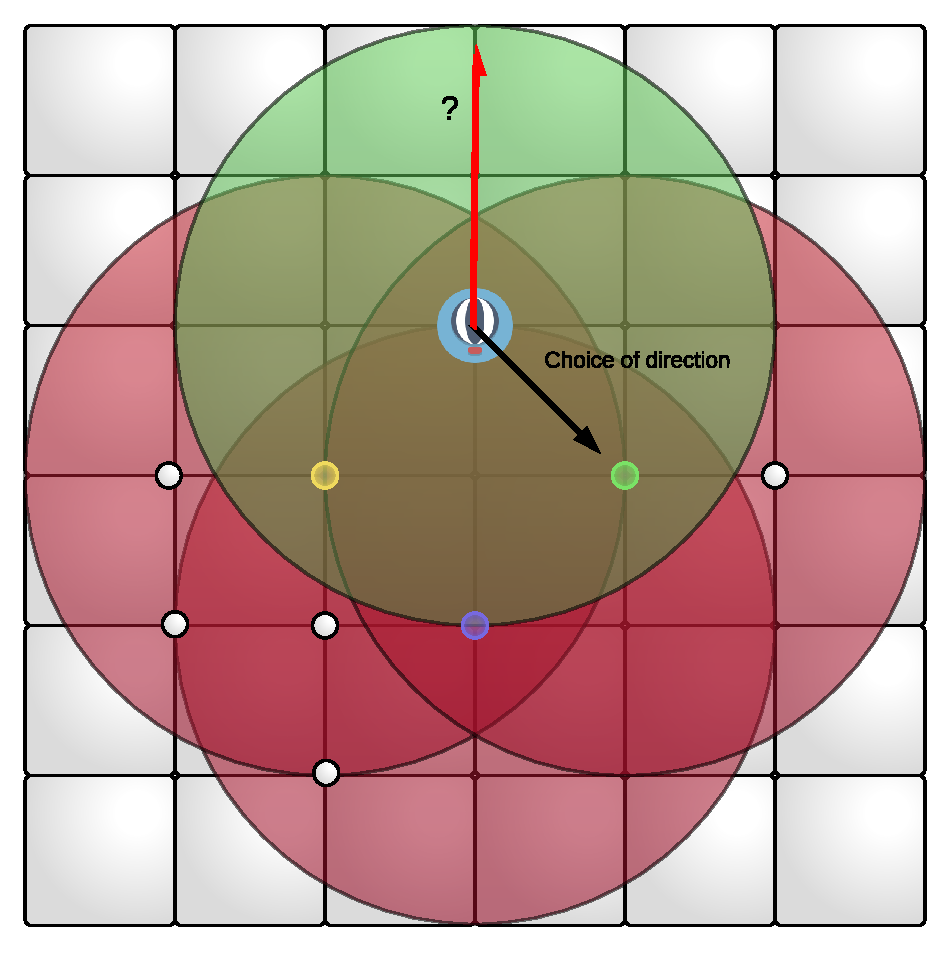
\includegraphics[scale = 0.3]{graphics/errorWithLogicCritical.pdf}
\caption{The problem is that the algorithm moves to the least occupied area, but not the empty area}
\label{fig:errorLogic}
\end{figure}

The flaw with the logic of Algorithm 3 and 4 is displayed in Figure \ref{fig:errorLogic}. As the balloon does not have access to every point on the grid, it makes its decision based on the neighbouring balloons. This means that the balloon will always navigate towards another balloon. This is a flaw when it comes to spreading, but an advantage as the balloons always need to be in contact with each other. 

\subsection{Algorithm 4s}
\begin{figure}
\centering
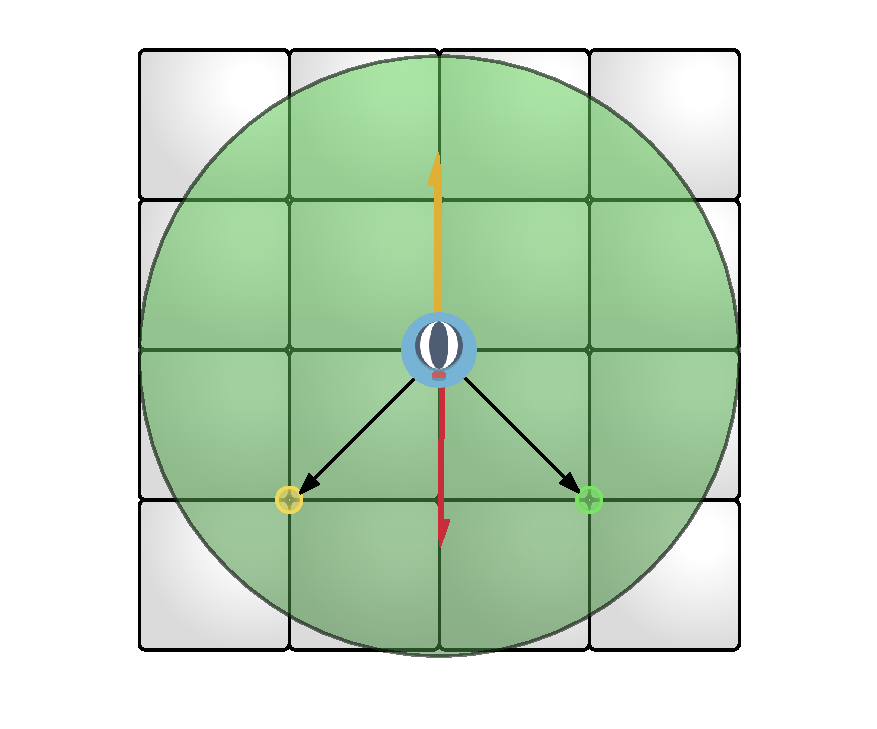
\includegraphics[scale = 0.3]{graphics/alg4s.pdf}
\caption{Algorithm 4s moves against all crowds}
\label{fig:alg4s}
\end{figure}

Like the $s$ suggests, Algorithm 4s is minor tweak of Algorithm 4. Like displayed in Figure \ref{fig:alg4s} this algorithm focuses on moving balloons away from all of their neighbours. This is done by adding the direction vectors from the balloon to each of the neighbours together, and computing the vector that points to the opposite direction. The movement to that particular direction is however still dependent on only the wind layers found in the neighbourhood. The balloon can still not choose perfectly its direction, but rather chooses between from a limited selection of wind layers.

\begin{algorithm}[H]
\ForAll{Balloon b : balloons}{
\If{b.age $<$ 50}{applyDecision1(b)}{}
\Else{
ArrayList n = find all neighbours\\

ArrayList w = all wind layers from n and b\\

Compute vector r (Red vector on figure \ref{fig:alg4s})\\

Create vector y (Yellow vector on figure \ref{fig:alg4s} )\\

Choose layer from w with direction closest to y. 
}}
\caption{Control Algorithm 4s}
\label{alg:4s}
\end{algorithm}


\begin{figure}[H]
\centering
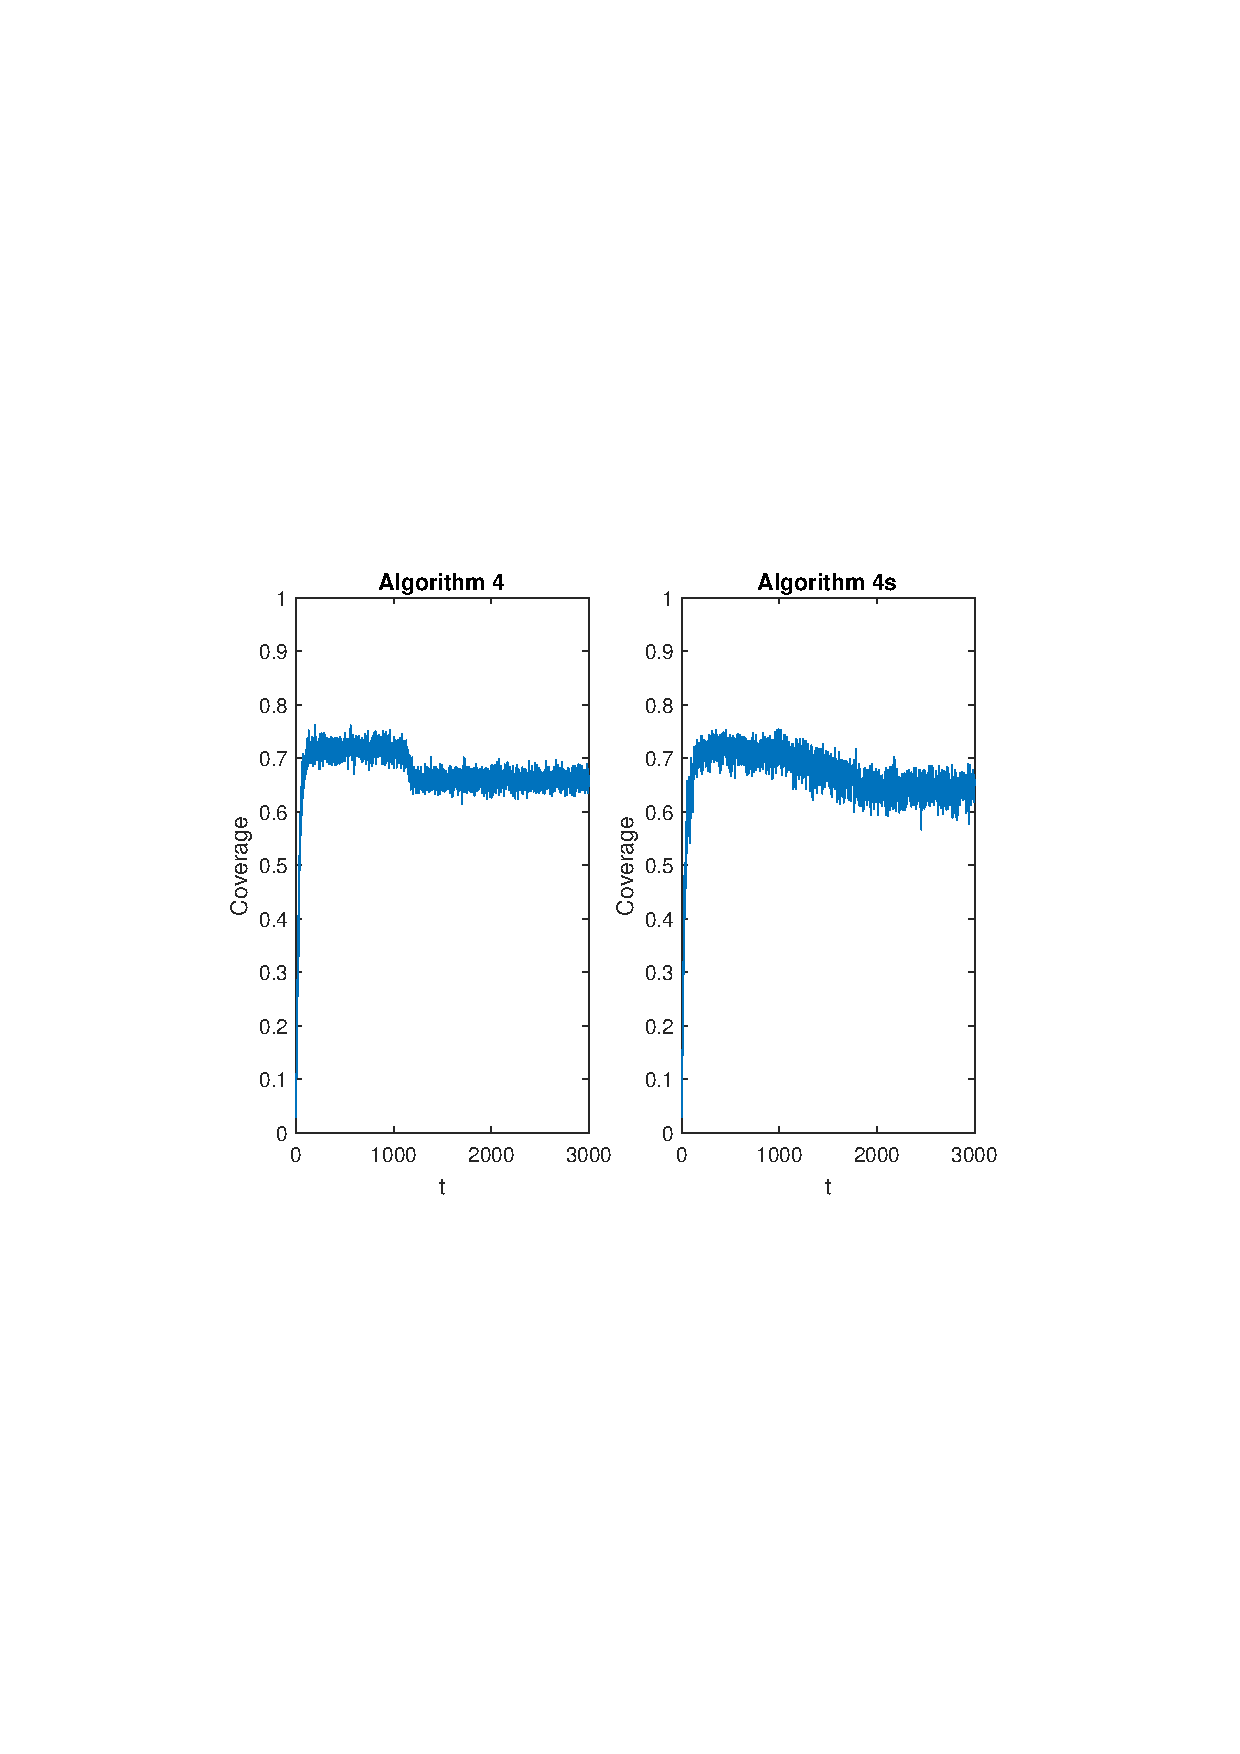
\includegraphics[scale=0.7, trim={3cm 10cm 4cm 9cm},clip]{graphics/coverage_alg4_vs_alg4s_3000_LONG.pdf}
\caption{Algorithm 4 vs. Algorithm 4s in 3000 steps with an infinite lifetime of each balloon}
\label{fig:alg4vsalg4s_long}
\end{figure}

\begin{figure}[H]
\centering
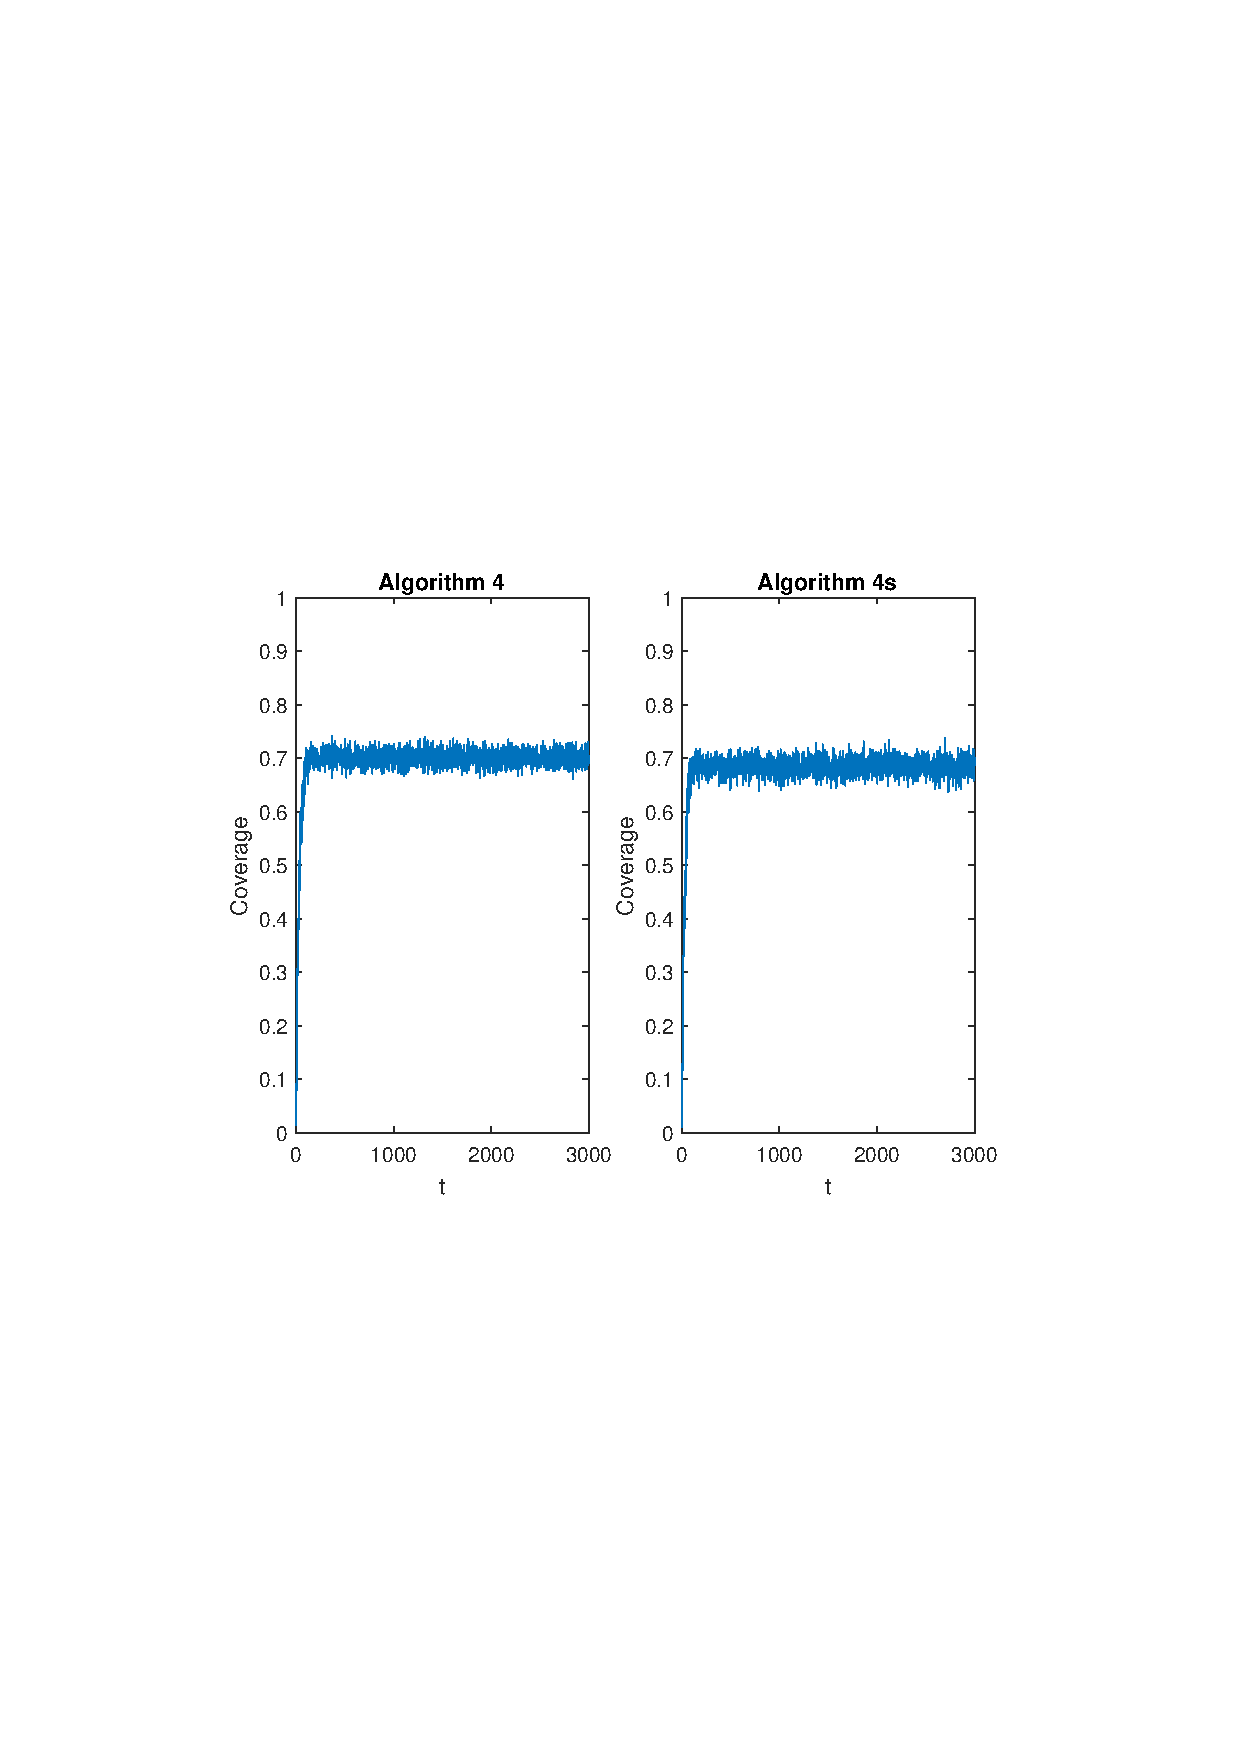
\includegraphics[scale=0.7, trim={3cm 10cm 4cm 9cm},clip]{graphics/coverage_alg4_vs_alg4s_3000_200.pdf}
\caption{Algorithm 4 vs. Algorithm 4s in 3000 steps with lifetime 200}
\label{fig:alg4vsalg4s_200}
\end{figure}

It is interesting to see that both Algorithm 4 and 4s both perform better when the balloon has a fixed lifetime. The coverage is stable and relatively similar. 

\begin{table}[]
\centering

\begin{tabular}{r|l|l|}

\textbf{Statistic}                 & \textbf{Algorithm 4} & \textbf{Algorithm 4s} \\ \hline
\textbf{Runtime (ms):}                  & 12610             & 9427                  \\ \hline
\textbf{Coverage over simulation:} & 69.5\%               & 67.9 \%               \\ \hline
\textbf{Dropped Connections:}      & 826.054              & 902.472               \\ \hline
\end{tabular}
\caption{Results. Algorithm 4 vs. 4s}
\label{tbl:res}
\end{table}

Table \ref{tbl:res} shows better the difference between the two, but Algorithm 4 has just slightly better coverage and more stable as well as it loses fewer connections during the simulation.